\chapter{Introduction to Flexibility Management and The Goal of This Thesis}
\chaptermark{Introduction}
%http://www.tex.ac.uk/FAQ-runheadtoobig.html
\label{ch:introduction}

\section{Defining flexibility and flexibility management}
\sectionmark{Definitions}
Maintaining balance between supply and demand is a fundamental requirement to electric power system operations. The capability of a power system to match the supply and demand at each point of time by using control resources are often referred to as ``operational flexibility", or simply ``flexibility" \cite{Cochran2014,Wang2017,Lund2015,Delft}. Flexibility is therefore not a new concept. Power systems are inherently with uncertainty and variability since loads vary over time and occasionally in unexpected ways, and power plants may suffer unpredictable failures sometimes. All power systems are designed and built with certain level of flexibility to cope with those unexpected events. Conventionally, the flexibility is mainly enabled on the supply side, where dispatchable resources are controlled to adjust their outputs to match the time-varying load.

However, following radical transformations towards decarbonization, decentralization and digitalization in the energy industry, the existing operating model of electricity flexibility is being critically challenged and increasing interests are moving to flexibility from the load side and energy storage technologies\cite{Lund2015,Bronski2015,McKinsey&Company2010}. These disruptions are not only in technological but also in institutional and managerial manners, which are sparking market restructures and business model innovations. For instance, those new resources are typically smaller in scale compared the traditional flexible generations so the new operating model shall be managed via more decentralized approaches. Flexibility management, as an emerging business term, refers to the process how those new small-to-medium scale sources of flexibility are enabled, organized and exploited to serve the needs of power systems.

\section{Challenges in power system flexibility}
\sectionmark{Challenges}
The penetration of renewable energy sources (RES), which is spreading over the whole industry globally \cite{Agency2016}, are commonly viewed as the fundamental driver for the transformation that is creating operational challenges in maintaining system balance with existing flexibility resources \cite{Cochran2014,Wang2017,Lund2015,FraunhoferIWES2015,Muller2016,Kwon2014,Kondziella2016,Papaefthymiou2016,Alizadeh2016,Bertsch2016}. The impacts of RES on electric power systems can be deduced from the instinct technological attributes of RES \cite{Kondziella2016,Edenhofer2013}:
\begin{itemize}
	\item RES is variable and often viewed as non-dispatchable since its output is determined by weather conditions, and furthermore
	\item RES is usually imperfectly predicted and specific power generation is uncertain until realization.
\end{itemize}

Effects of the property being non-dispatchable can be illustrated by introducing the concept of ``net load", also referred to as ``residual load", which equals the total system load minus the renewable generation so represents the load that needs to be served by non-RES resources\cite{Cochran2014,Muller2016,Ueckerdt2015}.

\begin{figure}[h!]
	\centering
	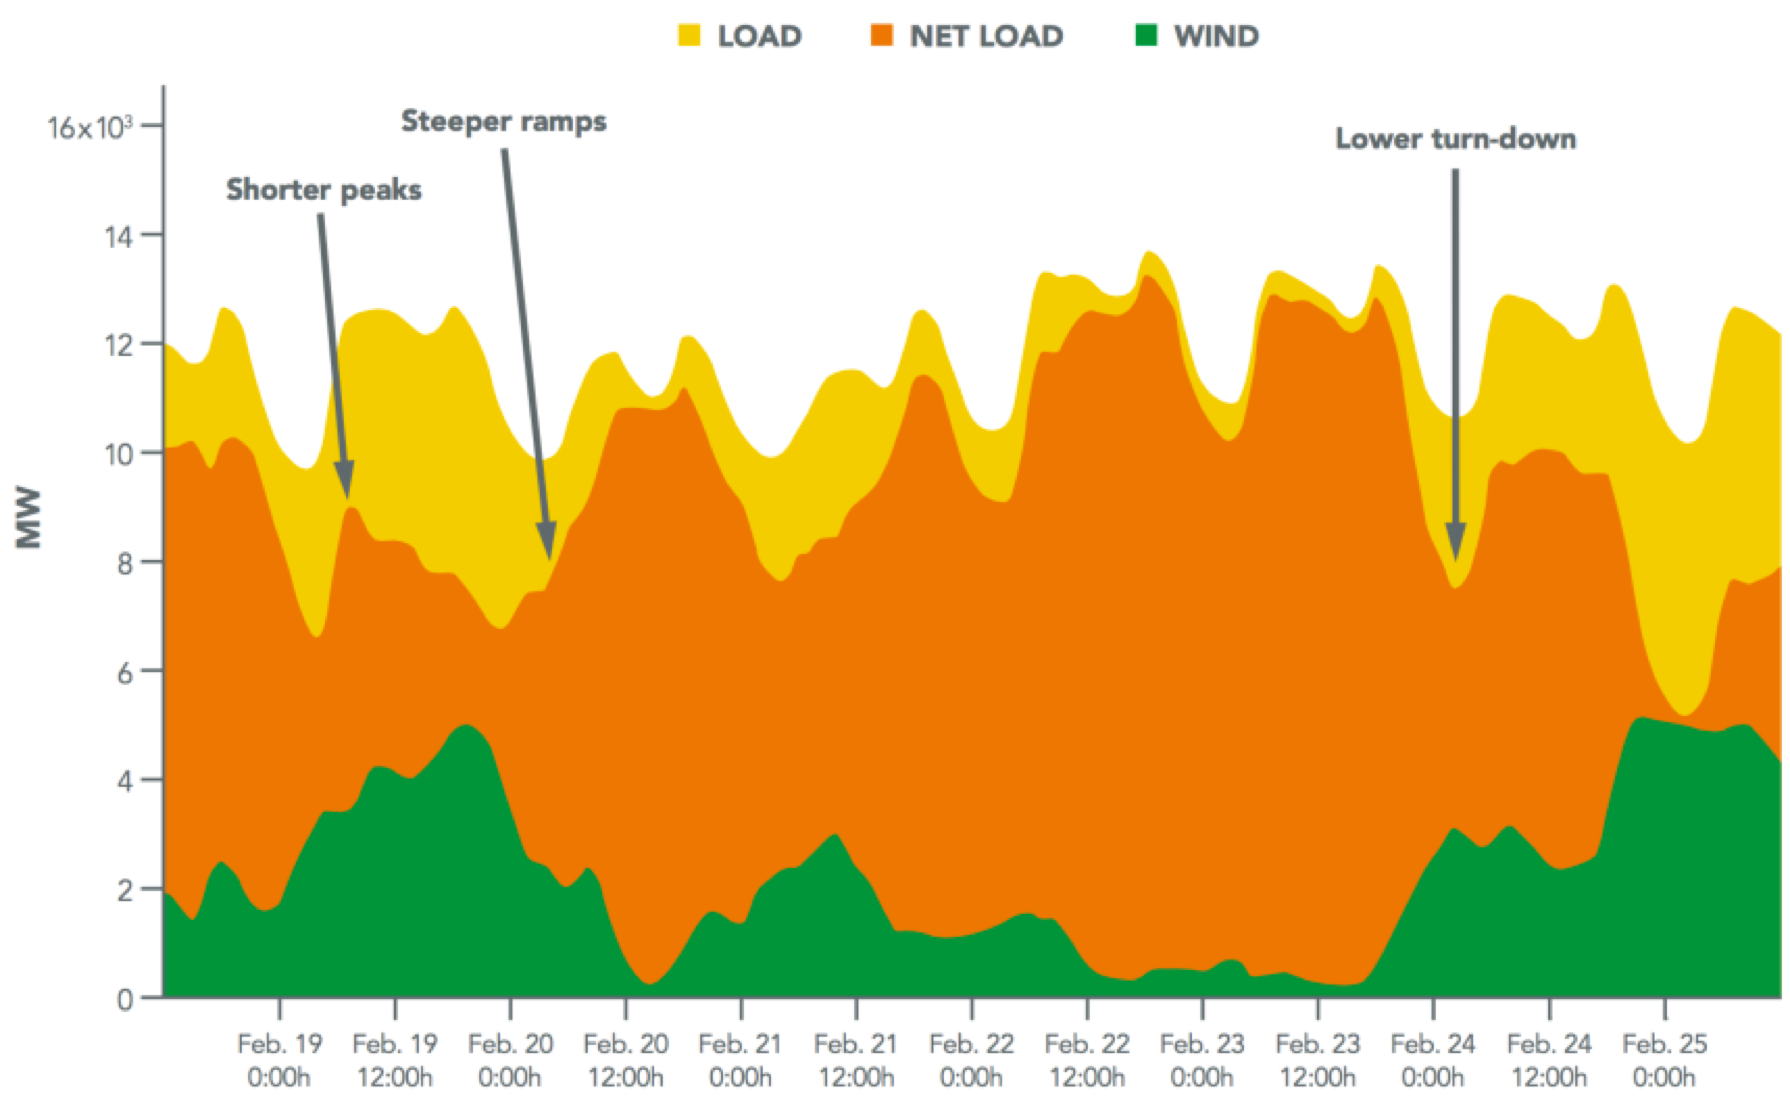
\includegraphics[width=0.9\linewidth]{Figures/NetLoad}
	\caption{An illustrative example of net load profile \cite{Cochran2014}}
	\label{fig:net-load}
\end{figure}

Figure \ref{fig:net-load} shows an example profile of net load, based on which we can see how RES is stressing the existing non-RES generations:

\begin{itemize}
	\item \textbf{Shorter peaks}: resulting in fewer operating hours for conventional peak generators, affecting their cost recovery and consequently long-term security of supply,
	\item \textbf{Lower turn-down}: diminishing the base load which was stable at a higher without RES, creating challenges to base generators who have limit operational flexibility to vary their outputs, and
	\item \textbf{Steeper ramps}: demanding higher performance in delivering flexibility, eliminating relative low-grade resources from serving the needs for flexibility.
\end{itemize}

It can be seen that the whole span of current generation portfolio serving base, flexible and peak power is under great pressure with the RES growth.

The issue of the forecast error, on the other hand, requires the dispatch of flexibility close to real-time operation. This is especially an explicit issue in places where those activities are organized through power markets. In present power markets, the major part of the scheduling and pre-dispatching is determined ahead of the operating day based on forecasts and errors deviated in real time from the schedule are mostly depending on imbalance settlements via so-call frequency control ancillary services which are typically more costly\cite{Ranci2013,Srivastava2011}. The intra-day market with higher resolution of price signals and shorter prediction horizon toward actual operation is a feasible option and implemented in many markets\cite{Srivastava2011} but intra-day markets are empirically prone to low liquidity in may regions \cite{Lund2015, Hagemann2015,Weber2010}. Without structural improvements in the market design, the demands for frequency control services would raise significantly and thus add burdens to the power system operators \cite{GEEnergyConsulting2014,Krad2017,Koch2009}. Measures such as improving day-ahead forecast \cite{Woo2016}, developing short-term frequency control product \cite{Gonzalez-Aparicio2015}, optimized intra-day \cite{Weber2010} and balancing market frameworks \cite{Wartsila2014}, have been proposed. Being sensitively depending on the market arrangements, existing businesses may be disrupted significantly by any of those market restructures.

Besides, solar power which is forecasted to have even higher potential than wind power in the long run is tending to grow in distributed patterns \cite{Agency2016,Epia2016,Sawyer2016}. With the conventional centralized deployment of flexibility, local congests are likely to exacerbate \cite{Lund2015,STEINKE2013826} which drives the needs for extensions of transmission and distribution capacity.

Collectively, the RES penetrations urge innovations in both technology and market design, which are otherwise burdening power system operators with higher expenses, potentially reducing the revenue scream of existing market players and/ or leading to significant curtailment of RES.

In addition to RES, the electrification of transportation, i.e. the penetration of plug-in electric vehicles (EV), is emerging more recently to be a second pole as the game changer. Facilitated by support policies by states or cities to uncap their multiple benefits such as transport decarbonization, air pollution reduction, and energy efficiency and security, the growth of EV has been accelerating significantly, having exceeded the global threshold of 2 million in 2016 \cite{InternationalEnergyAgency2017}. Although it tends to be treated as a promising source for flexibility by implementing vehicle to grid (V2G) technologies \cite{Size2016,Habib2015,Foley2013}, threats along with it shall not be ignored. Without being fully prepared in technologies and markets, the growth of EV may still move to the opposite side of flexibility with the negative impacts such as increasing peak demand and potential local congestion \cite{Green2011,DBLP:journals/corr/PournarasJZFS17}.

It has been pointed out that lack of flexibility can be identified more intuitively by signals such as \cite{Cochran2014,Wang2017}:
\begin{itemize}
	\item difficulty balancing demand and supply, resulting in frequency excursions or shedded load,
	\item significant renewable energy curtailments,
	\item negative market prices, and
	\item high price volatility in whole power markets.
\end{itemize}

Although having been discussed extensively for years in the academic area and by industry experts, it was not until quite recently when more and more signs of inflexibility had been witnessed did the public start to be indeed aware of the challenges on power system flexibility. For instance, the negative pricing in wholesale power spot market was first introduced in 2007 in Germany intra-day market and in 2008 in Germany/Australia day-ahead market\cite{EPEX_negative_price}, but vast attentions from the public were initiated after 146 hours on 24 days with negative prices were observed in the day-ahead market in 2017. Another famous example could be the power outage in South Australia that happened on September 28th 2016. After a widespread debate, Australia Energy Market Operator (AEMO) finally concluded in its investigation report that the generation deficit of wind farms due to unexpected operations of a control setting responding to multiple disturbances led to the power blackout  \cite{AEMO2016SA}.  This aroused public's worries on supply security from RES generation. As one of the follow-up actions, AEMO partnering with Tesla Inc., one of the leaders in global battery and electric vehicle markets,  built the worlds' largest battery energy storage system (BESS) in South Australia \cite{AEMO_tesla}.

These imply a proper timing for technology vendors to update their assessment on the market, as interests in flexibility management from the public and thus their potential customers have significantly raised.

\section{Technologies: options for system flexibility provision}
\sectionmark{Technologies}

Opportunities on flexibility management are not just being ignited by the increasing level of challenge but also being facilitated by the booming of innovations in technology. Thanks to significant developments in energy storage technologies and information communication technologies (ICT) in recent years, the landscape of flexibility options changed vastly. While it was in the past limited to centralized solutions, extracting flexibility from ubiquitous distributed resources and operating it in an aggregate way has been gradually becoming technically feasible and economical viable.

The availability of technological options to serve system flexibility has shown a great abundance which has never been seen in the past \cite{Cochran2014,Wang2017,Lund2015,Muller2016}. A systematic summary for these various possibilities can be found as Figure \ref{fig:TechnologyOptions}.

\begin{figure}[h!]
	\centering
	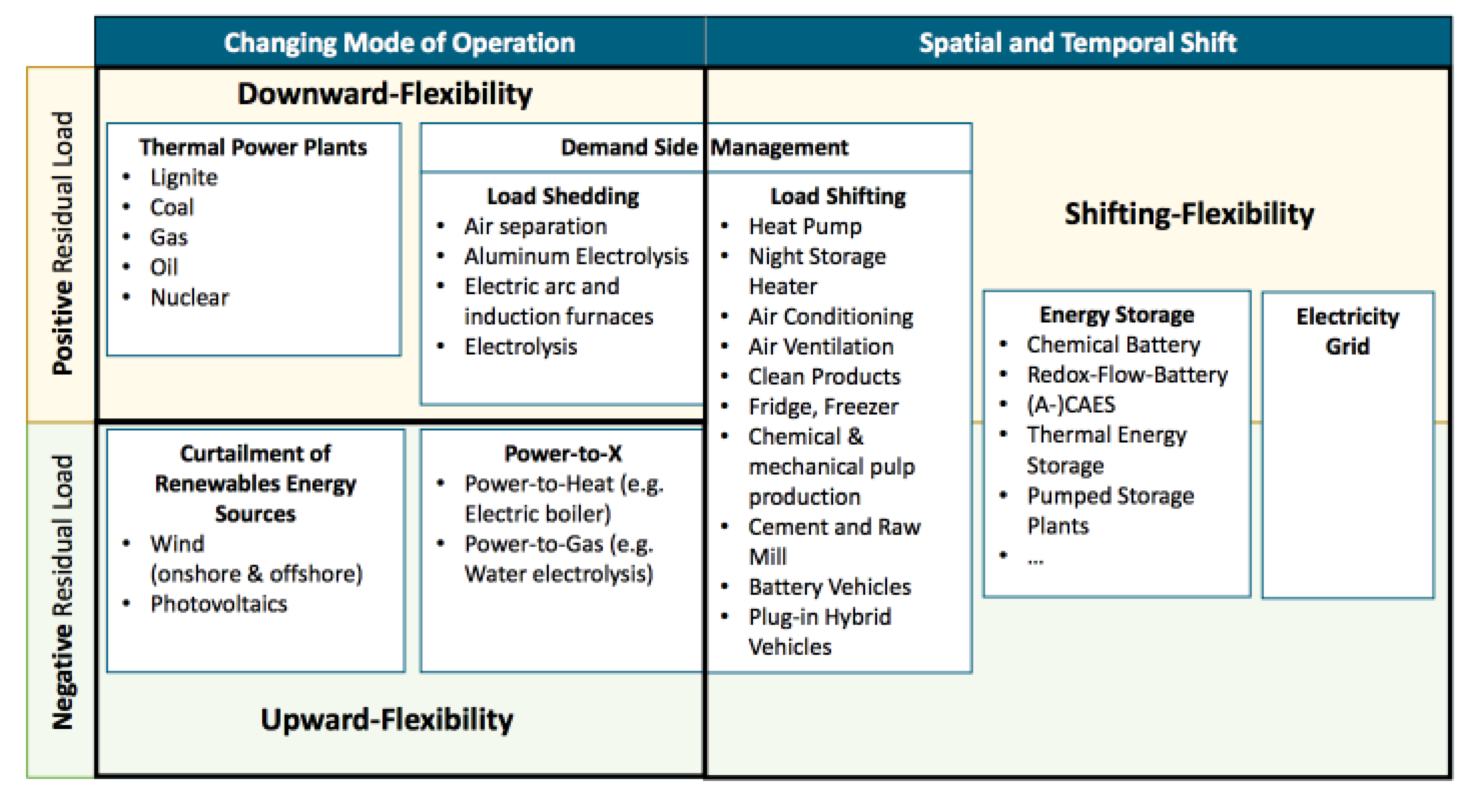
\includegraphics[width=0.95\linewidth]{Figures/TechnologyOptions}
	\caption{Overview flexibility options categorized in way of flexibility provision \cite{Muller2016}}
	\label{fig:TechnologyOptions}
\end{figure}

Technologies for flexibility are categorized by their type of provision:

\begin{itemize}
	\item \textbf{Downward-flexibility}: shedding demand or uplifting supply to reduce the positive residual load,
	\item \textbf{Upward-flexibility}: dropping surplus RES feed-in or increasing demand to mitigate negative residual load,
	\item  \textbf{Shifting-flexibility}: shuffling surplus energy from regions (or time steps) with negative or lower residual load to other regions (or time steps) and vice verse.
\end{itemize}

It can be clearly seen that the term demand-side management (DSM), or often referred to as demand response (DR), is actually a granular concept as an umbrella for a list of different technologies with many of them have totally disparate mechanisms. 

Combining the evaluations carried out by several studies \cite{Cochran2014,Wang2017,Lund2015,Muller2016,Despres2017}, the characteristics of different technologies can be summarized on a high level as:

\begin{itemize}
	\item \textbf{Generation}: i.e. flexibility provision by varying power plant outputs. 
	
	This is by far the most mature technology and typically not constrained by the duration of flexibility provision nor how often to be activated. Activation time and ramp rate are the main issues for flexibility from power plants, especially conventional power plants using stream turbines, e.g. coal, lignite and nuclear power plants. Although output adjustments can be done within 1 hour, a cold start may take up to 100 hours or at least 4 hours even by the state-of-the-art thermal power plants \cite{Muller2016,AgoraEnergiewende2017}. Gas turbines are more flexible even compared to some other advanced technologies that are to be introduced later, so they are deemed as a decent option to increase system flexibility \cite{Muller2016}.
	
	Cost is a complex topic and varies greatly between different type of generation technologies but in general they are still lower than most emerging technologies. However, building power plants is not a economical option to cover the extreme events that are rarely seen, as heavy fixed costs of building power plants can be hardly recovered in this scenario. Meanwhile, the issue related to consumption of fossil fuels and green house gas emission raise the uncertainty of operating costs in long term.
	
	\item \textbf{Load shedding}: i.e. load curtailment, mainly enabled by disrupting some energy-intensive industrial processes. In contrast to load shifting, shedded load will not be compensated later on as most of the time the industrial processes are running at their maximum allowances.
	
	Load shedding applications can provide fast responses, but are constrained at duration and numbers of activation. Nonetheless, short timespan of flexibility provision and limited occurrence fit the characteristics of extreme disturbances in power systems, so load shedding can be deployed for that specific purpose.
	
	The activation cost is essentially the loss caused by the disrupted productions so is indeed an adverse factor. The fixed cost, on the other hand, is less concerning as most industry plants nowadays are already equipped with automatic and intelligent energy management systems.
	
	\item \textbf{RES curtailment}: i.e. regulating the outputs of RES plants downwards.
	
	Technically, there are few constraints for RES curtailment as they can be performed promptly and frequently, and last for an indefinite time period. However, since curtailments will waive the revenues that otherwise be received by selling electricity in the market, RES operators are discouraged to do so. Although a list of measures that possible for power system operators to mandate curtailments, it is contradictory to the concept of decarbonization. 
	
	Therefore, we deem the RES curtailment as a compromise and the last option if the needs for flexibility cannot be fulfilled by any other means.
	
	\item \textbf{Power-to-X(P2X)}: i.e. consuming excess electricity to produce other energy carriers, e.g. hydrogen, methane or heat.
	
	P2X technologies can also provide fast response and theoretically last for an indefinite period of time. However, in reality it is virtually constrained by how the by-products are stored and utilized, and values of the by-products also vary significantly in different situations. For instance, while heat generation is valuable in winter, it is likely to be counterproductive in summer. 
	
	Regarding the cost, power-to-gas technologies requires significant high initial investments on equipment while power-to-heat costs much less less with the core components being boilers and heat tanks. Overall, the economics of P2X is still a challenging issue as the value can be harvested only if the by-products are competitive compared to goods by other production methods. However, production of P2X is destined to be intermittent as it would only be activated while upward-flexibility is needed, making it difficult to be economically viable.
	
	\item \textbf{Energy storage}: a system that can absorb surplus energy in time with negative or low residual while release energy in time with higher demand. Due to its technical nature, the energy storage can act on both supply and demand side or be viewed as a third pole \cite{Gunter2016}.
	
	Energy storage itself is a umbrella for an abundance of technologies, including battery energy storage systems (BESS), pumped hydroelectric storage (PHES), compressed air energy storage (CAES), flywheel, thermal storage, and others. These technologies vary significantly in their mechanism and thus in technical parameters such as size and efficiency as well as in performances, e.g. duration, action time, cost, etc. Among them, BESS could be the most attractive with fast response (activated within seconds), decent duration (up to 10 hours) and most importantly few external dependencies, like geographic conditions. Cost is the main concern for batteries, but is decreasing dramatically in recent year \cite{Nykvist2015}.
	
	%\cite{Rastler2010,Eyer2010}
	
	%\begin{itemize}
		%\item \textbf{Batteries} use electrochemical reactions, i.e. oxidation-reduction processes between the battery's electrolyte and electrodes, converting electricity to chemical energy stored and vice verse. Battery is one of the most focused areas in research and an increasing number of novel batteries are being developed. More familiar and mature ones include lead-acid, lithium-ion, sodium/sulfur (Na/S), and others. Flow batteries, sometimes
		%\item \textbf{\item{}}
	%\end{itemize}
	
	\item \textbf{Load shifting}: corresponding to the concept of demand response in a narrower sense where responsive loads are enabled by direct control signals or indirect price signals.
	
	There are a great variety of load types that can be exploited for load shifting, so similar to energy storage load shifting contains a list of subcategories. However, unlike other technologies that can be characterized by relative standard models, load shifting shows a higher diversity. This is because the characteristics of a load shifting system would be sensitively affected not only the technical parameters of load but also the control strategy and the users' preferences. Nonetheless, the load shifting in general has short activation time (within seconds to minutes), short duration (typically 0.5 to 8 hours) and relatively low cost (even close to zero if applications are equipped with control devices). 

	\item \textbf{Electricity grid}: i.e. extension of distribution and transmission capacity. Distinguishing other technologies discussed above that shuffle electricity temporarily, the grid extension is the only option that deals with fluctuations of residual load spatially. 
	
	Flexibility from transmission and distribution (T\&D) network has the fastest response, indefinite duration and unlimited numbers of activation so together with the generation flexibility it has been a main solution for conventional power system flexibility. However, challenges come from the development of distributed energy resources (DER) which are disrupting the existing T\&D systems with altered electricity flow profiles and congestion in the network is a major bottleneck for delivering flexible power in the grid. Further grid infrastructure upgrade is necessary but leads to exceptionally high expenses so should be complemented by other technologies introduced above \cite{Cochran2014}.
	
\end{itemize}

Studies reveal that an abundance of different flexible technologies will be available in the future, and it is well agreed that no single option would be sufficient to provide flexibility to power systems \cite{Cochran2014,Wang2017,Lund2015,Muller2016}. Determining the the best mix of options need to be carried out on a case base and requires significant efforts as being a complex technological-institutional-economic issue. 

The innovations in technology, changes on market frameworks and cost reductions will collectively change the landscape, and overall create more available options for players. Therefore, technology vendors shall keep watching the development of technologies and constantly update their view on which technologies to supply. 

\section{Applications, benefits and business models}
\sectionmark{Applications}
So far we have introduced the mega-trends with growing challenges and opportunities on power system flexibility. It is however not sufficient to understand the value of flexibility from a business-oriented point of view. More detailed analysis on applications, benefits and business models are necessary.

Here application means a use where flexibility is exploited for a certain aim via certain procedures. Benefit denotes a value that can be evaluated in monetary, financial or social terms. Business model describes the rationale of how the application-specific benefits are being captured by a certain business player.


 Generally, these three items are disparate in a liberated power market compared to a vertically integrated market.

\subsection{In liberalized market}


%\subsubsection{Needs of different plyaers}

Player * Market * Application


%\subsubsection{Energy Markets}


%\subsubsection{Ancillary Service Markets}

\subsection{In vertically integrated market}
(placeholder)
\newpage


\section{Scope and research questions}

\subsubsection{Scope of benefits}

Explicit revenue from power markets

\subsubsection{Scope of technology}

Firstly, we are focusing on small-to-medium scale emerging solutions in low-to-medium voltage level, so flexibility provisions from conventional generations and pumped hydro power plants are excluded. Electricity grid extension also falls into this category, plus its value is not accounted as explicit revenue in power markets, so it is also excluded.

Secondly, RES curtailment as is mentioned previously is consider as a compromise rather than opportunity. Moreover, the benefits of RES curtailment may be valued from a system point view for grid stability maintenance. It will usually lead to no increase on explicit revenue for the play from power markets that is of our interests, unless the RES operators are obligate to meet the schedule and published for deviations.

P2X are also excluded, because the values of its by-products such as hydrogen and heat are hard to account in a generic way and definitely not a explicit revenue from the power markets.

Load shedding is not an emerging technology with few opportunities for technology vendors. Besides, they depend on type of load and are not ...

Energy storage and DSM. DSM is too granular as is analyzed. Different specific system has its own dynamic. We take ESS and EV as special example of . 





The target audience of this thesis is the management at Landis+Gyr on a high coporate level.

The ultimate goal is to provide references to support the audiences' strategic decision makings regarding flexibility management.

In order to achieve this, we conducted qualitative studies and developed quantitative models to identify: 1) the value of markets for flexiblity management

\begin{itemize}
	\item 
\end{itemize}

The goal of this thesis is to:

developed a robust modeling tool with moderate complexity so that it can not only provide results in current environment but can be also reused or easily revised to provide results in case of changes in the future.

based on the tool, make quantitative as well as quanlitative analysis to provide refer 

Purpose: providing references for strategic decision makings regarding flexibility management.

In order to make the analysis robust and reliable, we have built a techno-economic models which include the bottom-up dynamics of some key elements regarding the electricity markets and flexilibity technologies. 

However, it shall be noticed this thesis is not intended to serve for:

project developers to design a flexiblity system or make operating (including bidding) strategies of the system

policy makers to redesign the electricity market structure, rules or other policies

grid planners to understand the needs and options of flexibility in order to acheive system relability with lowest costs


Since the concept of flexiblity management is related to a great variety of technologies, applications and Landis+Gyr is positioning globally in various markets, the scope could be very broad. Nonetheless, in order to produce viable and reliable results with a solidily established techno-economic model, we have to make comprises. According to the relevance to Landis+Gyr's business, the scopes are defined as:

%\subsection{Scope of technologies}

%\subsection{Scope of applications}

%\subsection{Scope of benefits and business models}
The potential business model of Landis+Gyr is either to supply products to the customers to help them enable flexibility or to directly sell them flexible MWs as a service. In this case, we want to understand the value of each MW we enabled or sold. We assume Landis+Gyr will not directly partipate and trade in the power market, as it is going to place Landis+Gyr at the rival side of some customers in that market.

The value of flexibility will definitely vary according to the purpose, users' portfolio and operating strategies. 


%\subsection{Scope of markets}